\section{Features}\label{jiveFeatures}
\begin{figure}[H]
	\centering
	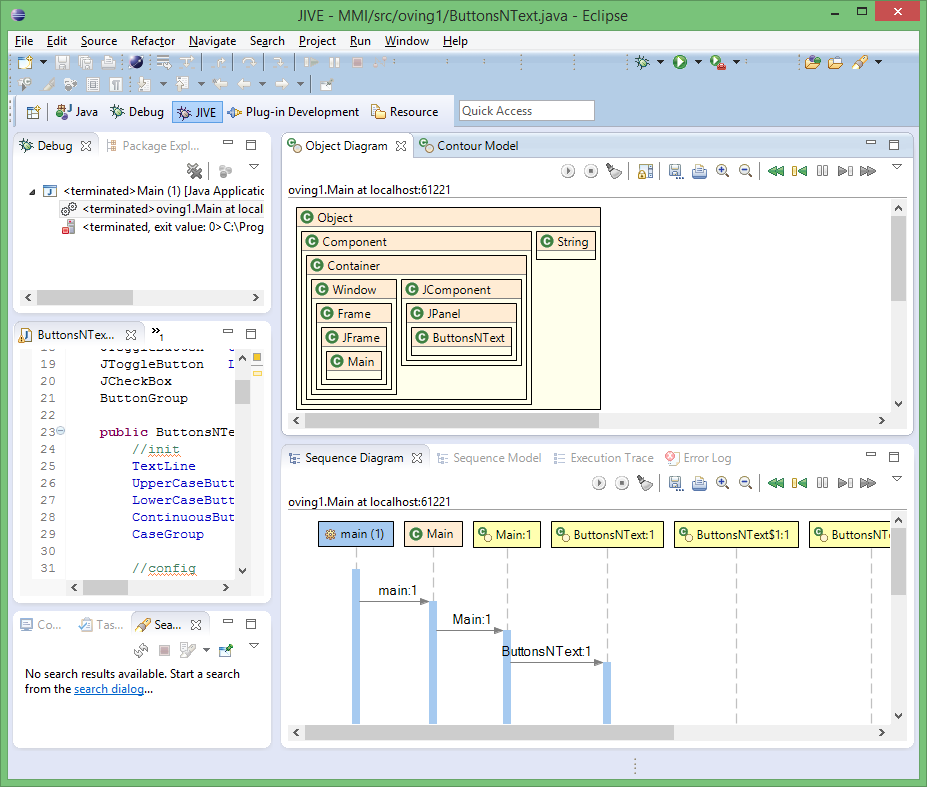
\includegraphics[width=\textwidth]{UIjivePerspective3}
	\caption{The JIVE perspective in Eclipse}
	\label{fig:UIjivePerspective}
\end{figure}

As mentioned in the prestudy, \gls{jive} installs as a plugin in the Eclipse IDE, adding another perspective in the environment shown in \cref{fig:UIjivePerspective}.
The default views shown in this perspective are the "object diagram" and "sequence diagram" views, making the diagrams that are generated during debugging the two most apparent features of \gls{jive}.
The diagrams are updated according to the current state of the debugged program, so that the backtracking functionality allows you to see the entire execution graphically step-by-step.
The other views provided by \gls{jive} are as follows: `contour model', `sequence model', `execution trace' and `search'.

\begin{figure}[H]
	\centering
	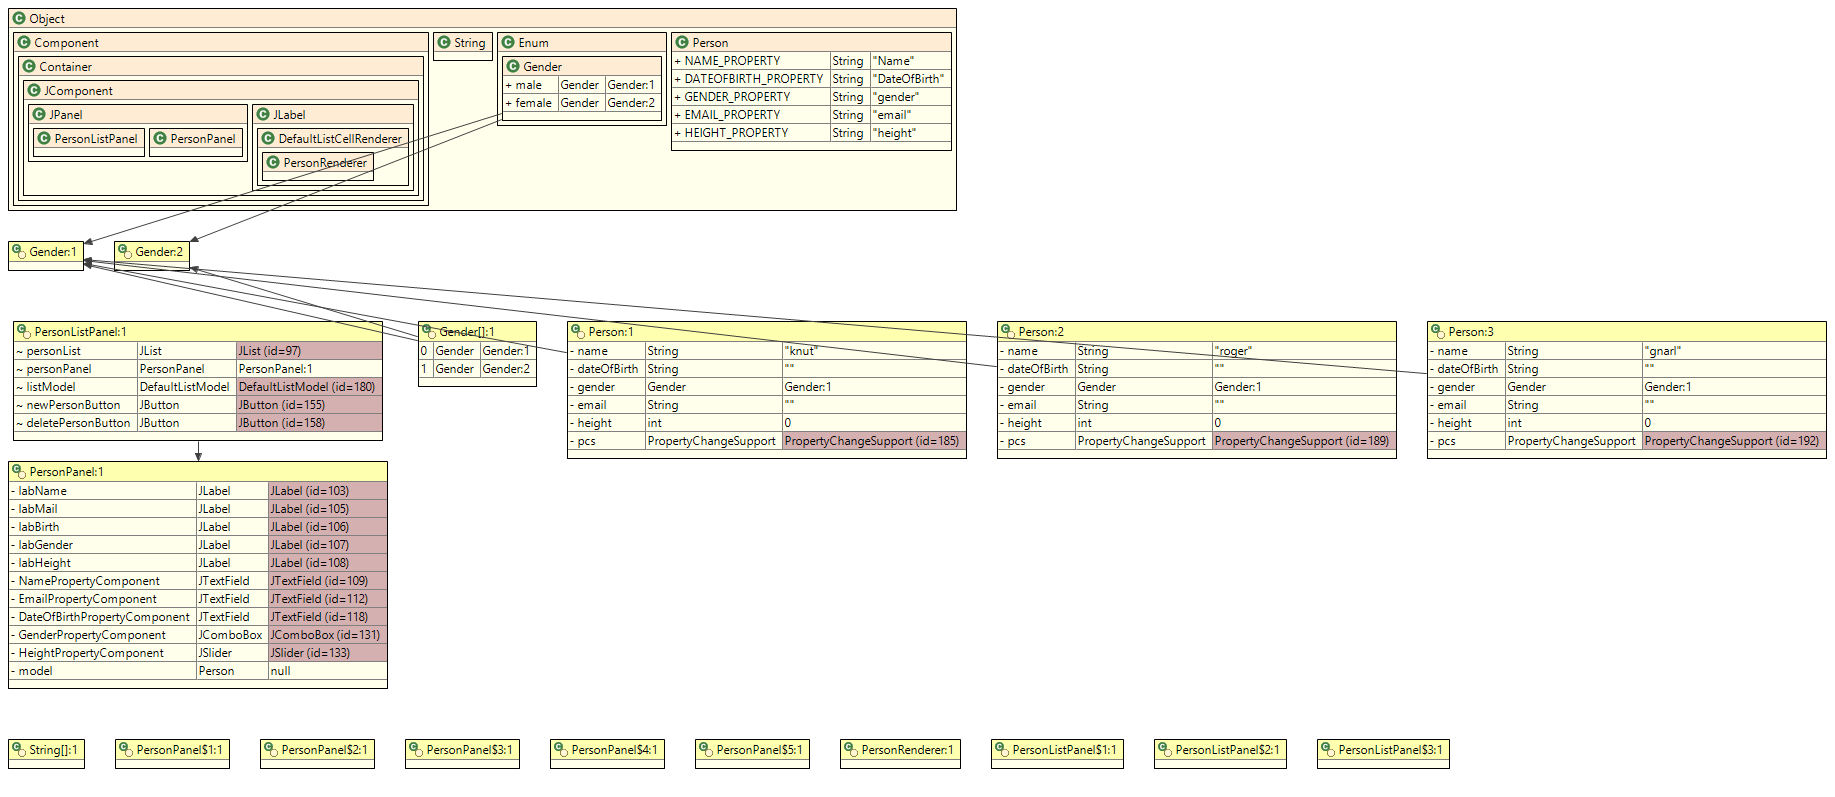
\includegraphics[width=\textwidth]{MMI-Oving4-ObjectDiagInit}
	\caption{A contour diagram generated by JIVE}
	\label{fig:contOving4Init}
\end{figure}

The object diagram-view shows the current state of the program by using a contour-diagram.
Contour-diagrams, as shown in \autoref{fig:contOving4Init}, are based on an old technique to give semantics to Algol-like languages.
The basis has been extended to support modern concepts, such as object-oriented programming, and can be compared to object diagrams, in terms of the information that is shown.
Objects are represented by a box, or contour.
Within the contour, the objects variables are shown, with name, type and value.
The contour also uses arrows to point at other contours that are related, e.g. an other object representing the value of a variable, or an enumerator.
Inheritance is shown by putting the contour of an object within the contour of the extended object. 
Object instances are kept separate from the contours representing inheritance, but will have relational links when necessary.
Method calls are also represented in the diagram, in their own contours, linked to the calling object.
\gls{jive} offers to hide some of the information, such as inheritance or the composition of objects, in order to make the diagram smaller, and easier to read.
This can be especially useful when working with larger programs that are composed of many objects and relations.
Visibility is aided by the use of colors to highlight specific elements of the diagram, such as variables bound to objects, and method-calls.


\begin{figure}[H]
	\centering
	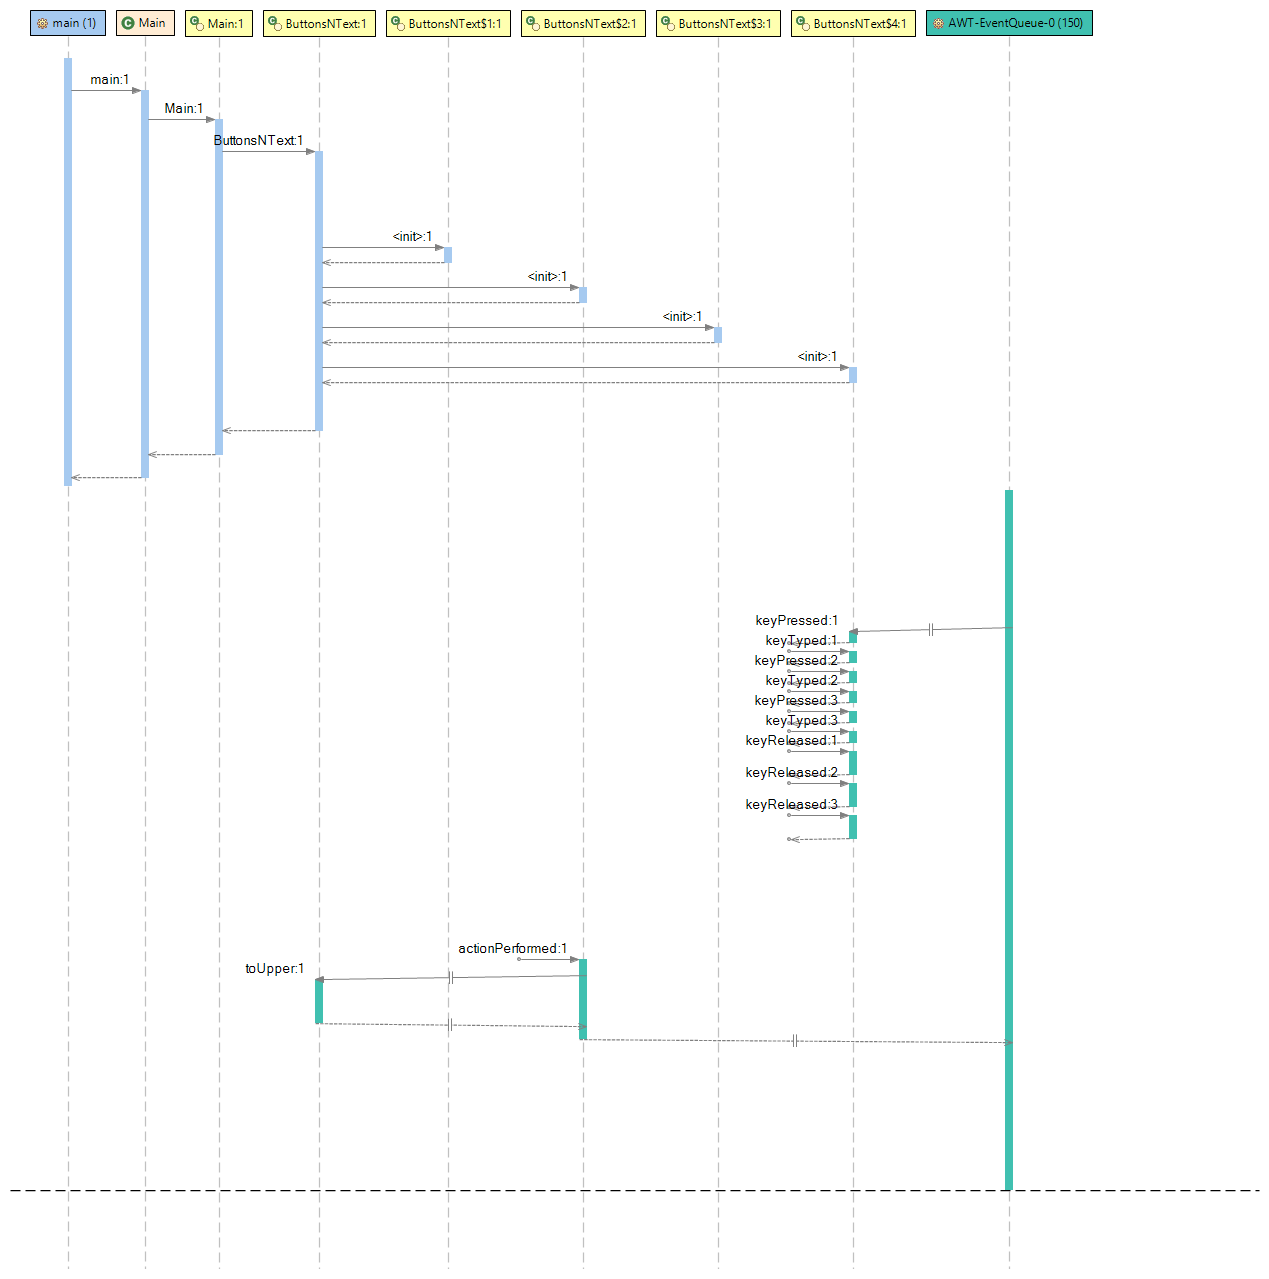
\includegraphics[width=\textwidth, trim=0 0cm 0 0, clip]{MMI-Oving1-SequenceDiag}
	\caption{A sequence diagram generated by JIVE, while running an instance of HCI-Exercise 1}
	\label{fig:seqOving1}
\end{figure}
The sequence diagrams, shown in \autoref{fig:seqOving1}, are fairly standard, with threads and object instances represented by boxes in a row at the top, each with a vertical line coming down.
The actual process is shown with a thicker lifeline overlaying the vertical line of the object that is currently active, with arrows between lifelines representing method-calls.
In order to differentiate the threads where the execution is happening, the sequences are colored with the same color as the thread- box the sequence originates from, regardless of which objects and methods are involved.
In \autoref{fig:seqOving1}, one can clearly see the two colors representing the main- and the AWT-event-thread, and how elements in the diagram are colored by their parent thread.
\begin{figure}[H]
	\centering
	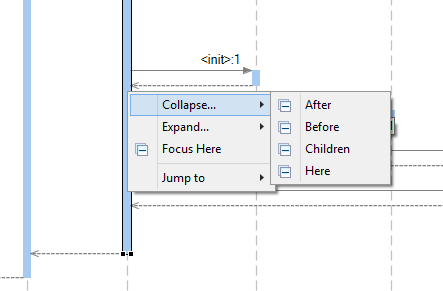
\includegraphics[scale=0.9]{UIseqRightClick}
	\caption{The sequence diagram right click menu}
	\label{fig:UIseqRightClick}
\end{figure}
Right-clicking on a lifeline provides the ability to collapse method-calls originating from that lifeline in order to hide unnecessary information, as shown in \autoref{fig:UIseqRightClick}.
The collapse-menu gives four options when used on the lifeline of an object: after, before, children and here.
`Before' and `after' collapses lifelines that occurred before or after the selected event, at the same depth in the sequence-tree.
`Children' collapses all events that are children of the selected event, while `here' collapses the selected event.
Right clicking on an object instance at the top of the diagram also gives the opportunity to collapse that object's entire lifeline, the result of which can be seen in \autoref{fig:seqOving4Collapse}.
While \autoref{fig:seqOving4Collapse} shows the result of collapsing the lifeline of an object, a similar result can be achieved by selecting `collapse children' at the parent lifeline, or by selecting `collapse here' on each of the three method-calls shown.
The same options are available for expanding collapsed elements.
Right-clicking also provides to set the execution-state via the jump-option, updating the contour-diagram and -model to show that state.


\begin{figure}[H]
	\centering
	\begin{subfigure}{\textwidth}
		\centering
		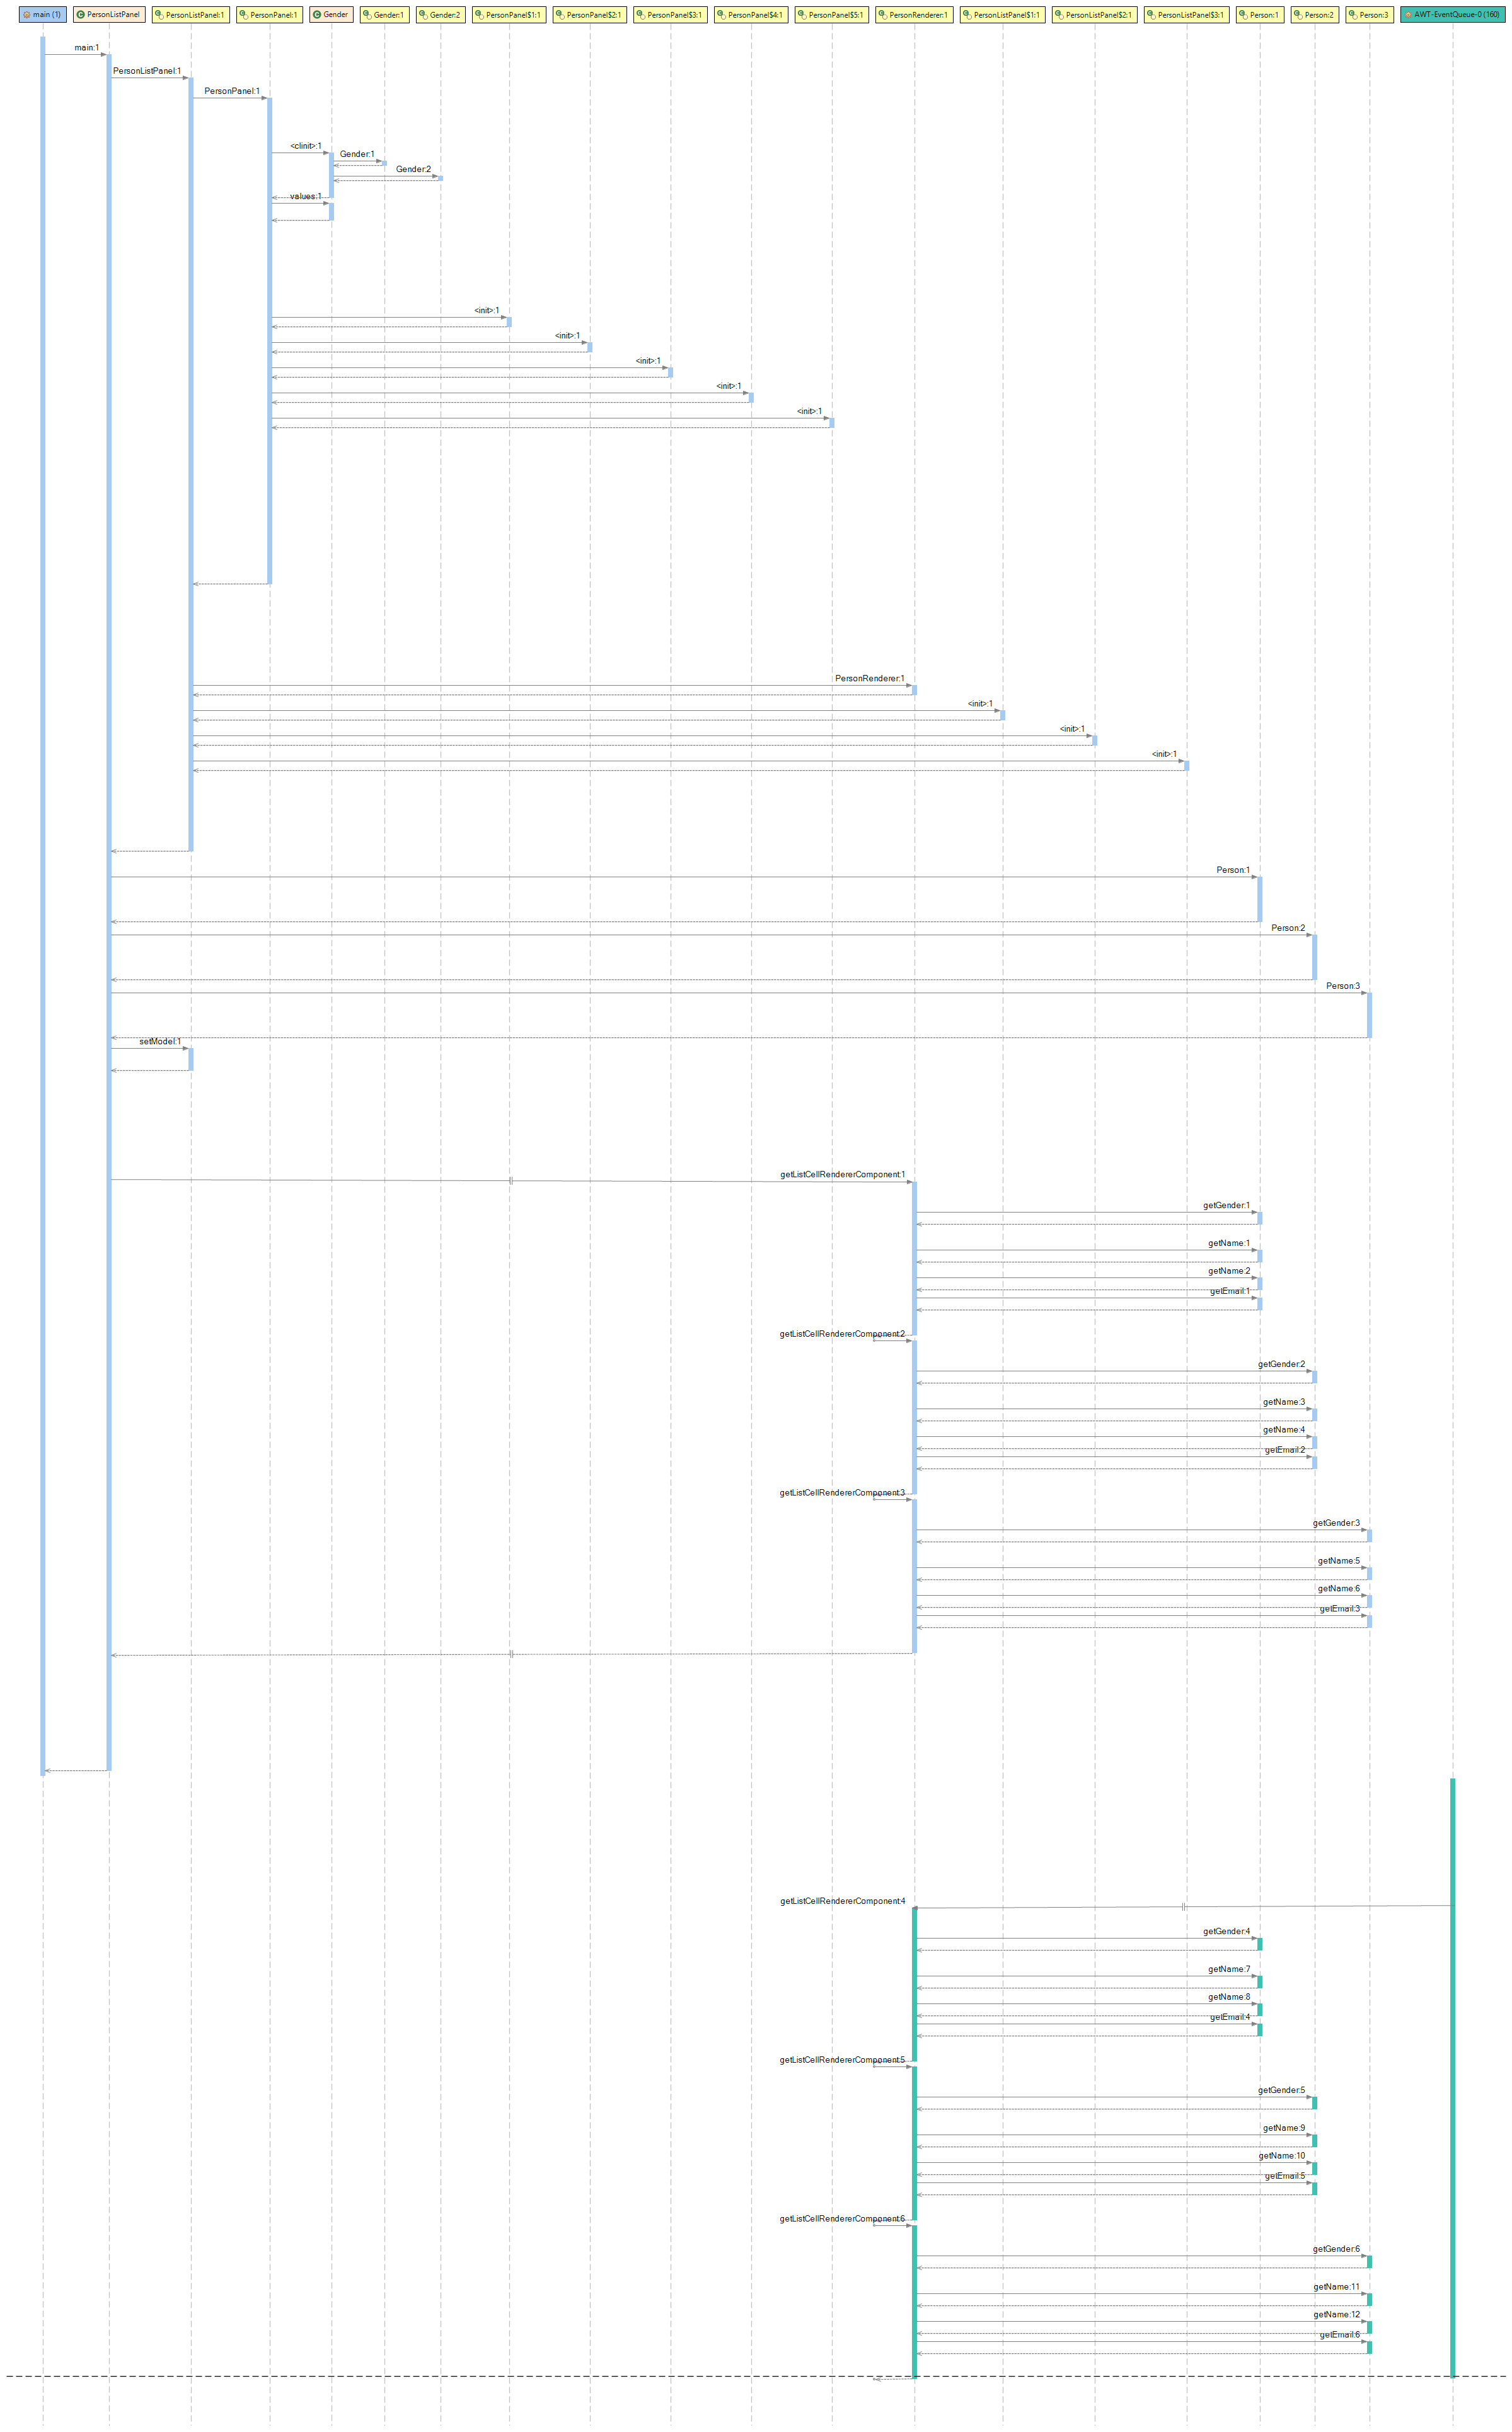
\includegraphics[width=\textwidth, trim= 30cm 48cm 10cm 65cm, clip]{MMI-Oving4-SequenceDiagInit}
		\caption{Normal}
		\label{fig:seqOving4CollapseA}
	\end{subfigure}
	\begin{subfigure}{\textwidth}
		\centering
		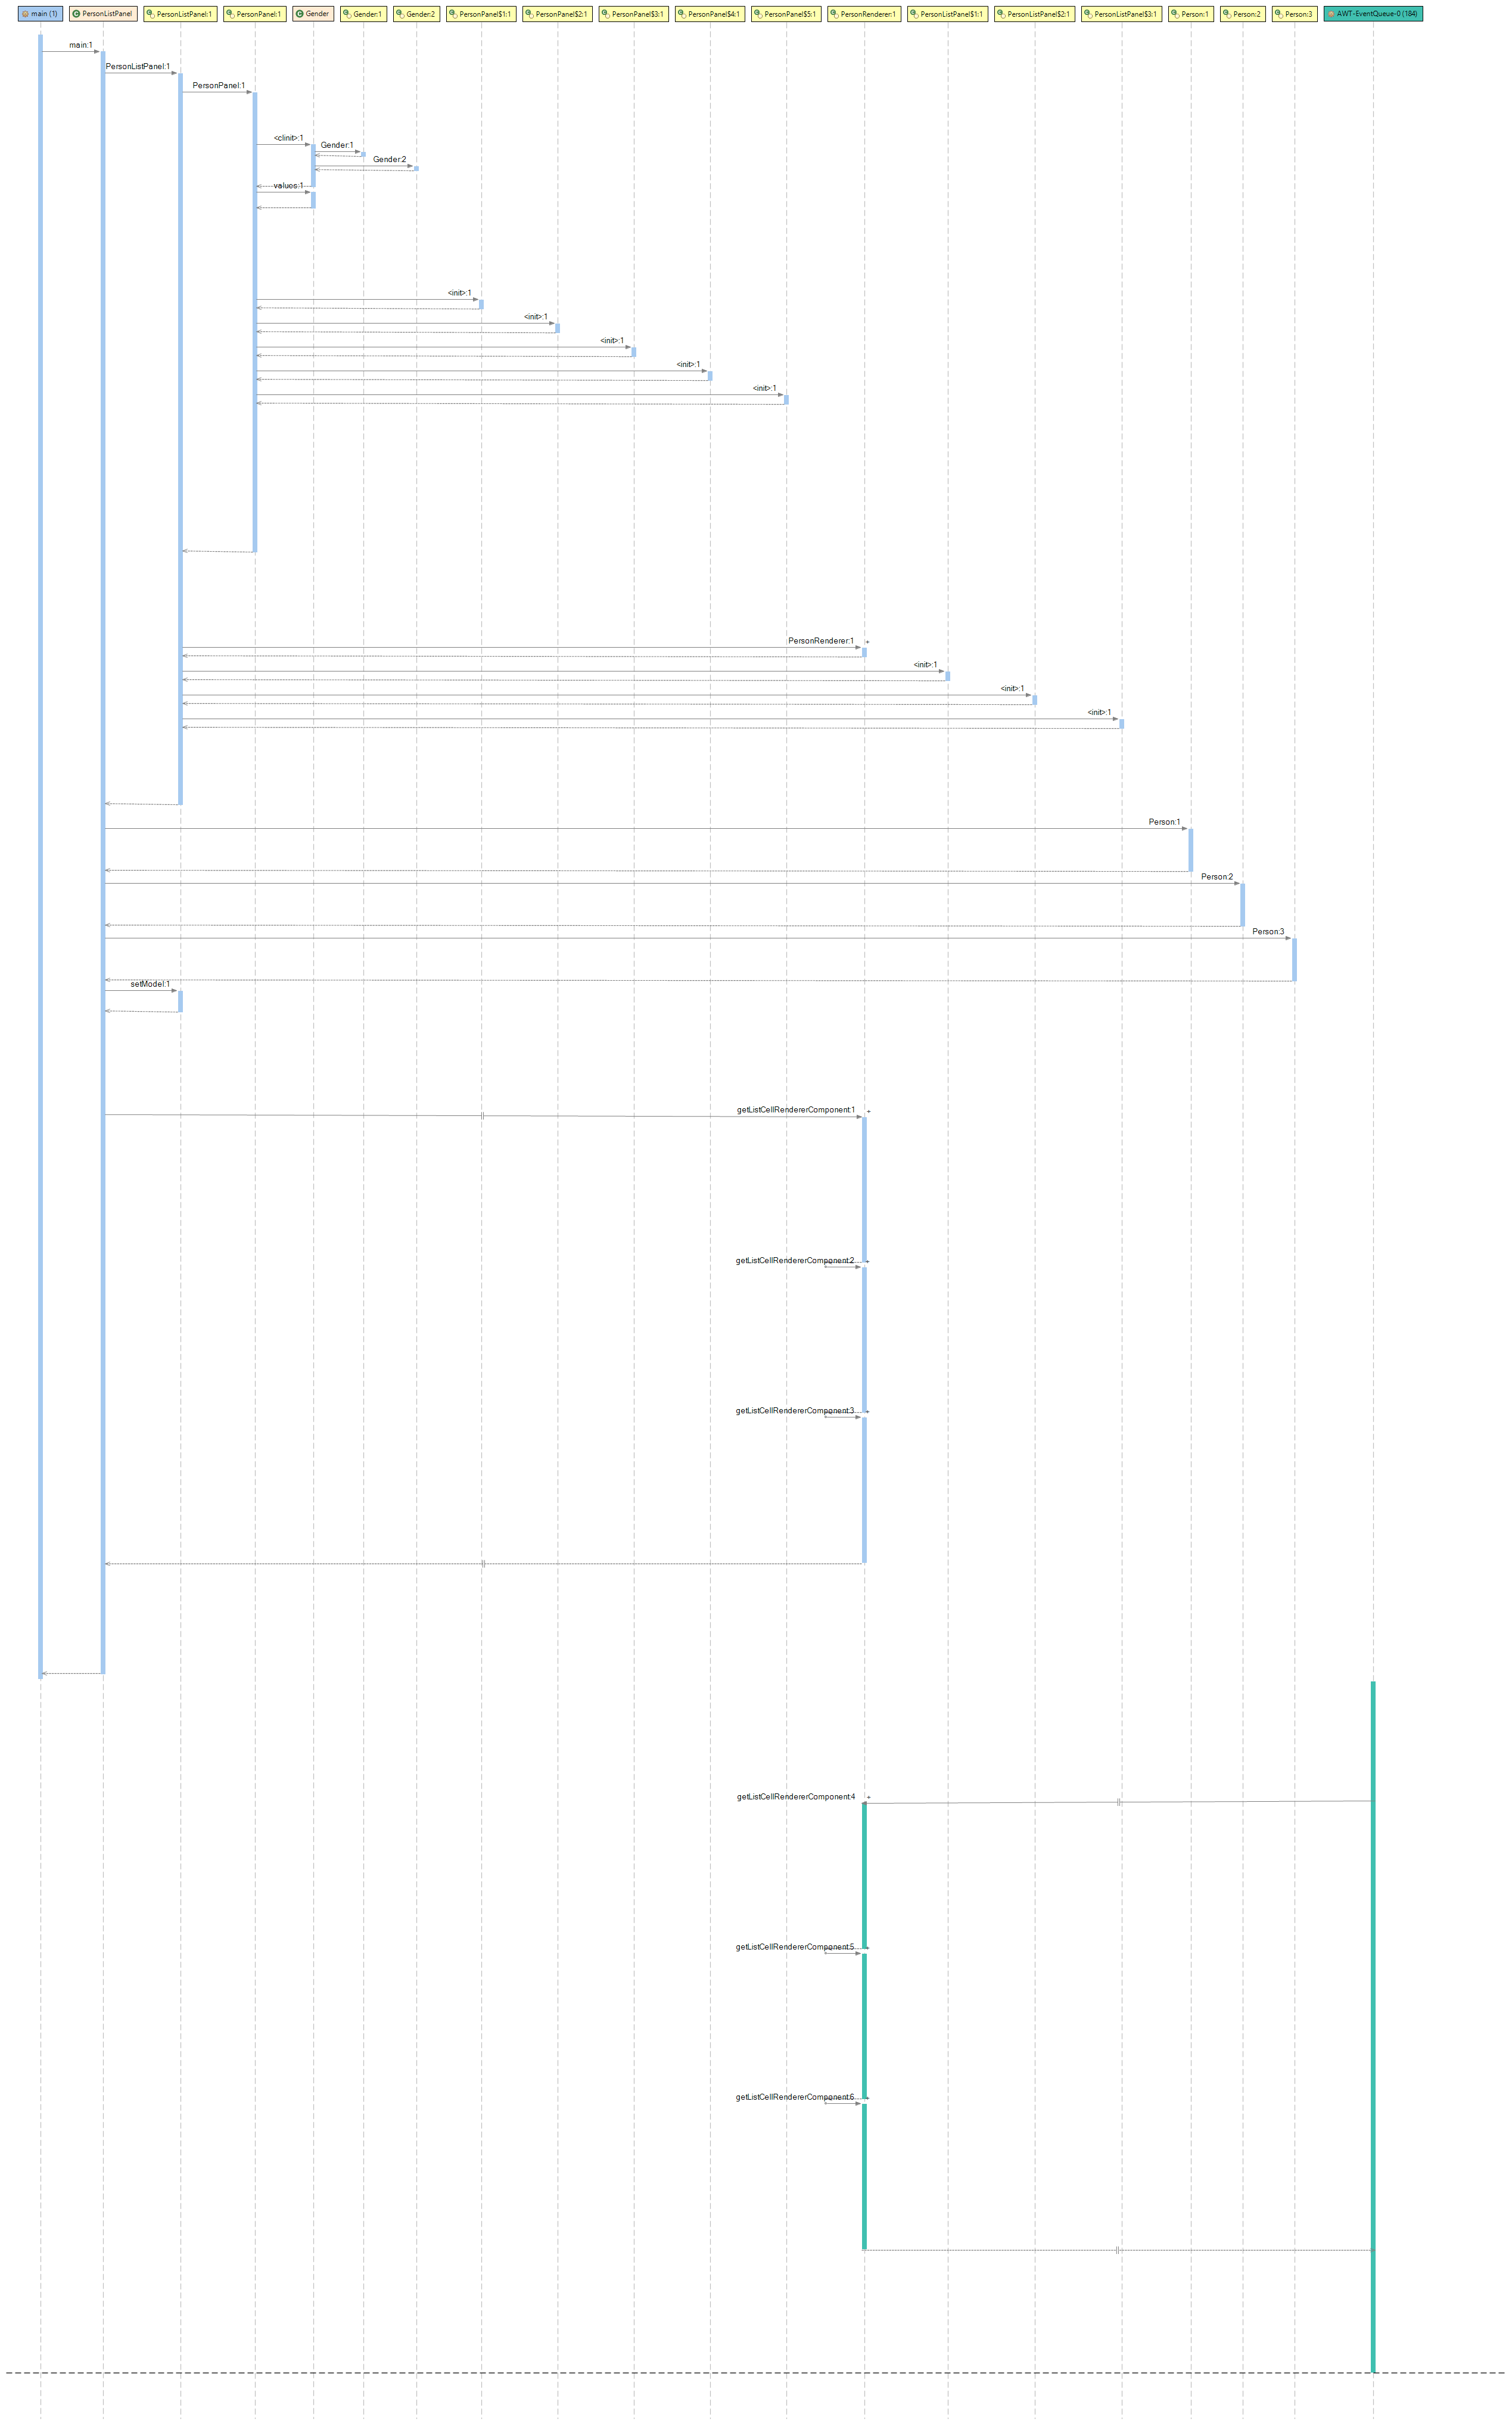
\includegraphics[width=\textwidth, trim= 30cm 48cm 10cm 65cm, clip]{MMI-Oving4-SequenceDiagInitCollapsed}
		\caption{Collapsed}
		\label{fig:seqOving4CollapseB}
	\end{subfigure}
	\caption{Normal and collapsed section of a sequence diagram}
	\label{fig:seqOving4Collapse} 
\end{figure}

Both of the diagrams can be saved as a high-resolution image at any time, so that one can look at diagrams from earlier runs, instead of being forced to view them through \gls{jive}.
This also helps to visualize any changes made to a program, and to see what the effects are on the program flow.
The diagrams also share the ability to zoom in and out, further helping with the handling of larger diagrams.

Closely related to the diagrams, is the ability to quickly jump backwards and forwards between execution states.%figur, jump-to
This is enabled by the trace-log, which contains an entry for every single event that occurs during the execution of a program, excluding those that are removed by the exclusion filter.
Each event is assigned an identifying number, in ascending order, and information about thread, type, caller, target, and the location of the source-code is stored.
The log is used as the basis for the models that make up the diagrams, and can be saved as both \gls{xml}- and \gls{csv}-files for later use.
As mentioned in the prestudy, logging every event has a significant impact on run-time performance, limiting the size and complexity of the programs that can be used with \gls{jive} in a meaningful way.
On the other hand, it allows quick jumping between recorded states, as opposed to techniques that save a snapshot at predefined intervals, requiring the program to be run from the snapshot-state to the desired one, even if it is just a single step backwards.

In order to improve both performance and readability, the mentioned exclusion filter checks the origin of each event, and determines whether or not the event is to be logged.
By default, the filter excludes the entire Java API, and by doing so, it focuses on the classes that are made by the user.%figur som viser filter?
This filter can be adjusted to better suit the program being analyzed, by adding or removing entries in order to show or hide details of the execution.

The model-views each display an alternate view of their respective diagrams.%figur begge modellvisninger, eventuelt vise begge modeller + logg
They show the data-model representing the diagrams in a hierarchical structure, much like the organization of files and folders.
Right-clicking on an event in the sequence model allows you to set the execution state to that event, and have the diagrams updated accordingly.
Clicking on elements in the contour-model allows you to inspect the values of objects and their variables.

Finally, the trace-log enables the use of queries to search for specific events in the execution.
The queries are presented through a new tab in the Eclipse search-window as seen in \autoref{fig:UIjiveSearchPanel}, easily accessible through the search-view, and comes with several pre-defined templates to simplify searching.
For example, searching for when a variable gets a certain value, only requires the user to specify the variable-name, the object it is contained within, and the value.
\begin{figure}[H]
	\centering
	\includegraphics[width=\textwidth]{UIjiveSearch}
	\caption{The JIVE search panel}
	\label{fig:UIjiveSearchPanel}
\end{figure}

